% topic: geometry
\question กำหนดให้มุม $\angle BAD = \angle CED$ และส่วนของเส้นตรง $\overline{AB} $ ขนานกับส่วนของเส้นตรง $\overline{EC} $ จงหาความยาวของส่วนของเส้นตรง $\overline{BC} $   
\begin{center}
    % เมื่อใช้งานจริงให้เปลี่ยนบรรทัดล่างนี้เป็นบรรทัดเรียกรูปภาพ เช่น: \includegraphics[width=0.35\textwidth]{image1.png}
    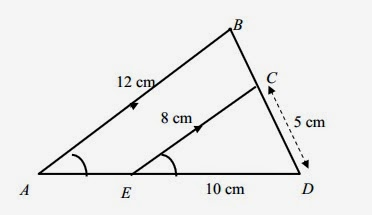
\includegraphics[width=0.35\textwidth]{triangle_problem.jpg}
\end{center}
\choicesgrid{2.5}{5}{7.5}{15}
% answer: 1